\documentclass[a4paper,11.5pt]{article}
\usepackage[textwidth=170mm, textheight=230mm, inner=20mm, top=20mm, bottom=30mm]{geometry}
\usepackage[normalem]{ulem}
\usepackage[utf8]{inputenc}
\usepackage[T1]{fontenc}
\PassOptionsToPackage{defaults=hu-min}{magyar.ldf}
\usepackage[magyar]{babel}
\usepackage{amsmath, amsthm,amssymb,paralist,array, ellipsis, graphicx,float}
%\usepackage{marvosym}

\makeatletter
\renewcommand*{\mathellipsis}{%
	\mathinner{%
		\kern\ellipsisbeforegap%
		{\ldotp}\kern\ellipsisgap%
		{\ldotp}\kern\ellipsisgap%
		{\ldotp}\kern\ellipsisaftergap%
	}%
}
\renewcommand*{\dotsb@}{%
	\mathinner{%
		\kern\ellipsisbeforegap%
		{\cdotp}\kern\ellipsisgap%
		{\cdotp}\kern\ellipsisgap%
		{\cdotp}\kern\ellipsisaftergap%
	}%
}
\renewcommand*{\@cdots}{%
	\mathinner{%
		\kern\ellipsisbeforegap%
		{\cdotp}\kern\ellipsisgap%
		{\cdotp}\kern\ellipsisgap%
		{\cdotp}\kern\ellipsisaftergap%
	}%
}
\renewcommand*{\ellipsis@default}{%
	\ellipsis@before
	\kern\ellipsisbeforegap
	.\kern\ellipsisgap
	.\kern\ellipsisgap
	.\kern\ellipsisgap
	\ellipsis@after\relax}
\renewcommand*{\ellipsis@centered}{%
	\ellipsis@before
	\kern\ellipsisbeforegap
	.\kern\ellipsisgap
	.\kern\ellipsisgap
	.\kern\ellipsisaftergap
	\ellipsis@after\relax}
\AtBeginDocument{%
	\DeclareRobustCommand*{\dots}{%
		\ifmmode\@xp\mdots@\else\@xp\textellipsis\fi}}
\def\ellipsisgap{.1em}
\def\ellipsisbeforegap{.05em}
\def\ellipsisaftergap{.05em}
\makeatother

\usepackage{hyperref}
\hypersetup{
	colorlinks = true	
}

\DeclareMathOperator{\Int}{int}
\DeclareMathOperator{\tg}{tg}
\DeclareMathOperator{\ctg}{ctg}
\DeclareMathOperator{\Th}{th}
\DeclareMathOperator{\sh}{sh}
\DeclareMathOperator{\ch}{ch}
\DeclareMathOperator{\sgn}{sgn}
\DeclareMathOperator{\arc}{arc}
\DeclareMathOperator{\arctg}{arc tg}
\DeclareMathOperator{\arcctg}{arc ctg}

\begin{document}
	%%%%%%%%%%%RÖVIDÍTÉSEK%%%%%%%%%%
	\setlength\parindent{0pt}
	\def\s{\hspace{0.2mm}\vphantom{\beta}}
	\def\Z{\mathbb{Z}}
	\def\Q{\mathbb{Q}}
	\def\R{\mathbb{R}}
	\def\C{\mathbb{C}}
	\def\N{\mathbb{N}}
	\def\Ra{\overline{\mathbb{R}}}
	
	\def\sume{\displaystyle\sum_{n=1}^{+\infty}}
	\def\sumn{\displaystyle\sum_{n=0}^{+\infty}}
	
	\def\narrow{\underset{n\rightarrow+\infty}{\longrightarrow}}
	\def\limn{\displaystyle\lim_{n\to +\infty}}
	\def\limx{\displaystyle\lim_{x\to +\infty}}
	
	
	\theoremstyle{definition}
	\newtheorem{theorem}{Tétel}[subsection] 
	
	\theoremstyle{definition}
	\newtheorem{definition}[theorem]{Definíció} 
	\newtheorem{example}[theorem]{Példa} 
	\newtheorem{task}[theorem]{Feladat} 
	\newtheorem{note}[theorem]{Megjegyzés}
	\newtheorem{revision}[theorem]{Emlékeztető}
	%%%%%%%%%%%%%%%%%%%%%%%%%%%%%%%%%%%%%%%%%%%%%%%%%%%%%%%%%%%%%%%%%%%%%
	\begin{center}
		{\LARGE\textbf{Analízis II.}}
		
		{\Large Előadás jegyzet}
		
		11. óra.
	\end{center}
	A jegyzetet \textsc{Umann} Kristóf készítette Dr. \textsc{Szili} László  előadásán. (\today)
	
	%Külön köszönet jár \textsc{Csonka} Szilviának a képek elkészítésért.
	%\bigskip
	
	Tantárgyi honlap: \url{http://numanal.inf.elte.hu/~szili/Oktatas/An2_BSc_2016/index_An2_2016.htm}
	\section{Információk}
	
	
	\begin{compactitem}
		\item Második zh időpontja: dec. 16 (péntek) 19.00-21.00
		\item Harmadik zh időpontja: dec. 22 (csüt) 8.00-10.00
		\item Negyedik zh időpontja: jan 3 (kedd) 8.00-10.00
		\item zh-k előtt nem sokkal kint lesz a bizonyítással várt tételek listája
	\end{compactitem}
	
	\section{Határozott integrál (folyt.)}
	
	\begin{revision}
		$$f\in R[a,b]\quad \Rightarrow\quad \forall\varepsilon>0,\quad \exists\tau\in\mathcal{F}[a,b]:\quad \varOmega(f,\tau)=S(f,\tau)-s(f,\tau)<\varepsilon. $$
	\end{revision}
	\begin{theorem}
		Tegyük fel, hogy $f,g\in K[a,b]$
		\[ \left.\begin{gathered}
			\exists f\in R[a,b]\\
			\exists A\subset[a,b] \ \text{ \textbf{véges} halmaz}\\
			f(x)=g(x)\quad (\forall x\in[a,b]\setminus A)
		\end{gathered}\right\}\quad \Rightarrow\quad g\in R[a,b]\quad \text{és}\quad \int_a^bg=\int_a^bf \]
		\textit{bizonyítása meggondolandó.}
	\end{theorem}
	\begin{theorem}
		(műveleti tételek)
		
		Tegyük fel, hogy $f,g\in R[a,b]$.
		\begin{enumerate}
			\item $\forall \lambda, \mu\in\R:\quad \lambda f+\mu g\in R[a,b]\quad \text{és}\quad \int_a^b(\lambda f + \mu g)=\lambda\int_a^b f+\mu\int_a^bg$ 
			
			(az integrált lineáris)
			\item $f\cdot g\in R[a,b]$
			\item ha még: $\exists m>0:\quad |g(x)|>m\quad (\forall x\in[a,b])\quad \Rightarrow\quad \frac{f}{g}\in R[a,b]$
		\end{enumerate}
		\textit{bizonyítása meggondolandó.}
	\end{theorem}
	\subsection{Az integrál intervallum szerinti additivitás}
	
	\begin{theorem}
		Tegyük fel, hogy $f\in R[a,b],\quad \text{és}\quad c\in(a,b)$ tetszőleges. Ekkor:
		\[ f\in R[a,c],\quad f\in R[c,b]\quad \text{és}\quad \int_a^b=\int_a^cf+\int_c^bf \]
	\end{theorem}
	
	\begin{figure}[!h]
		\centering
		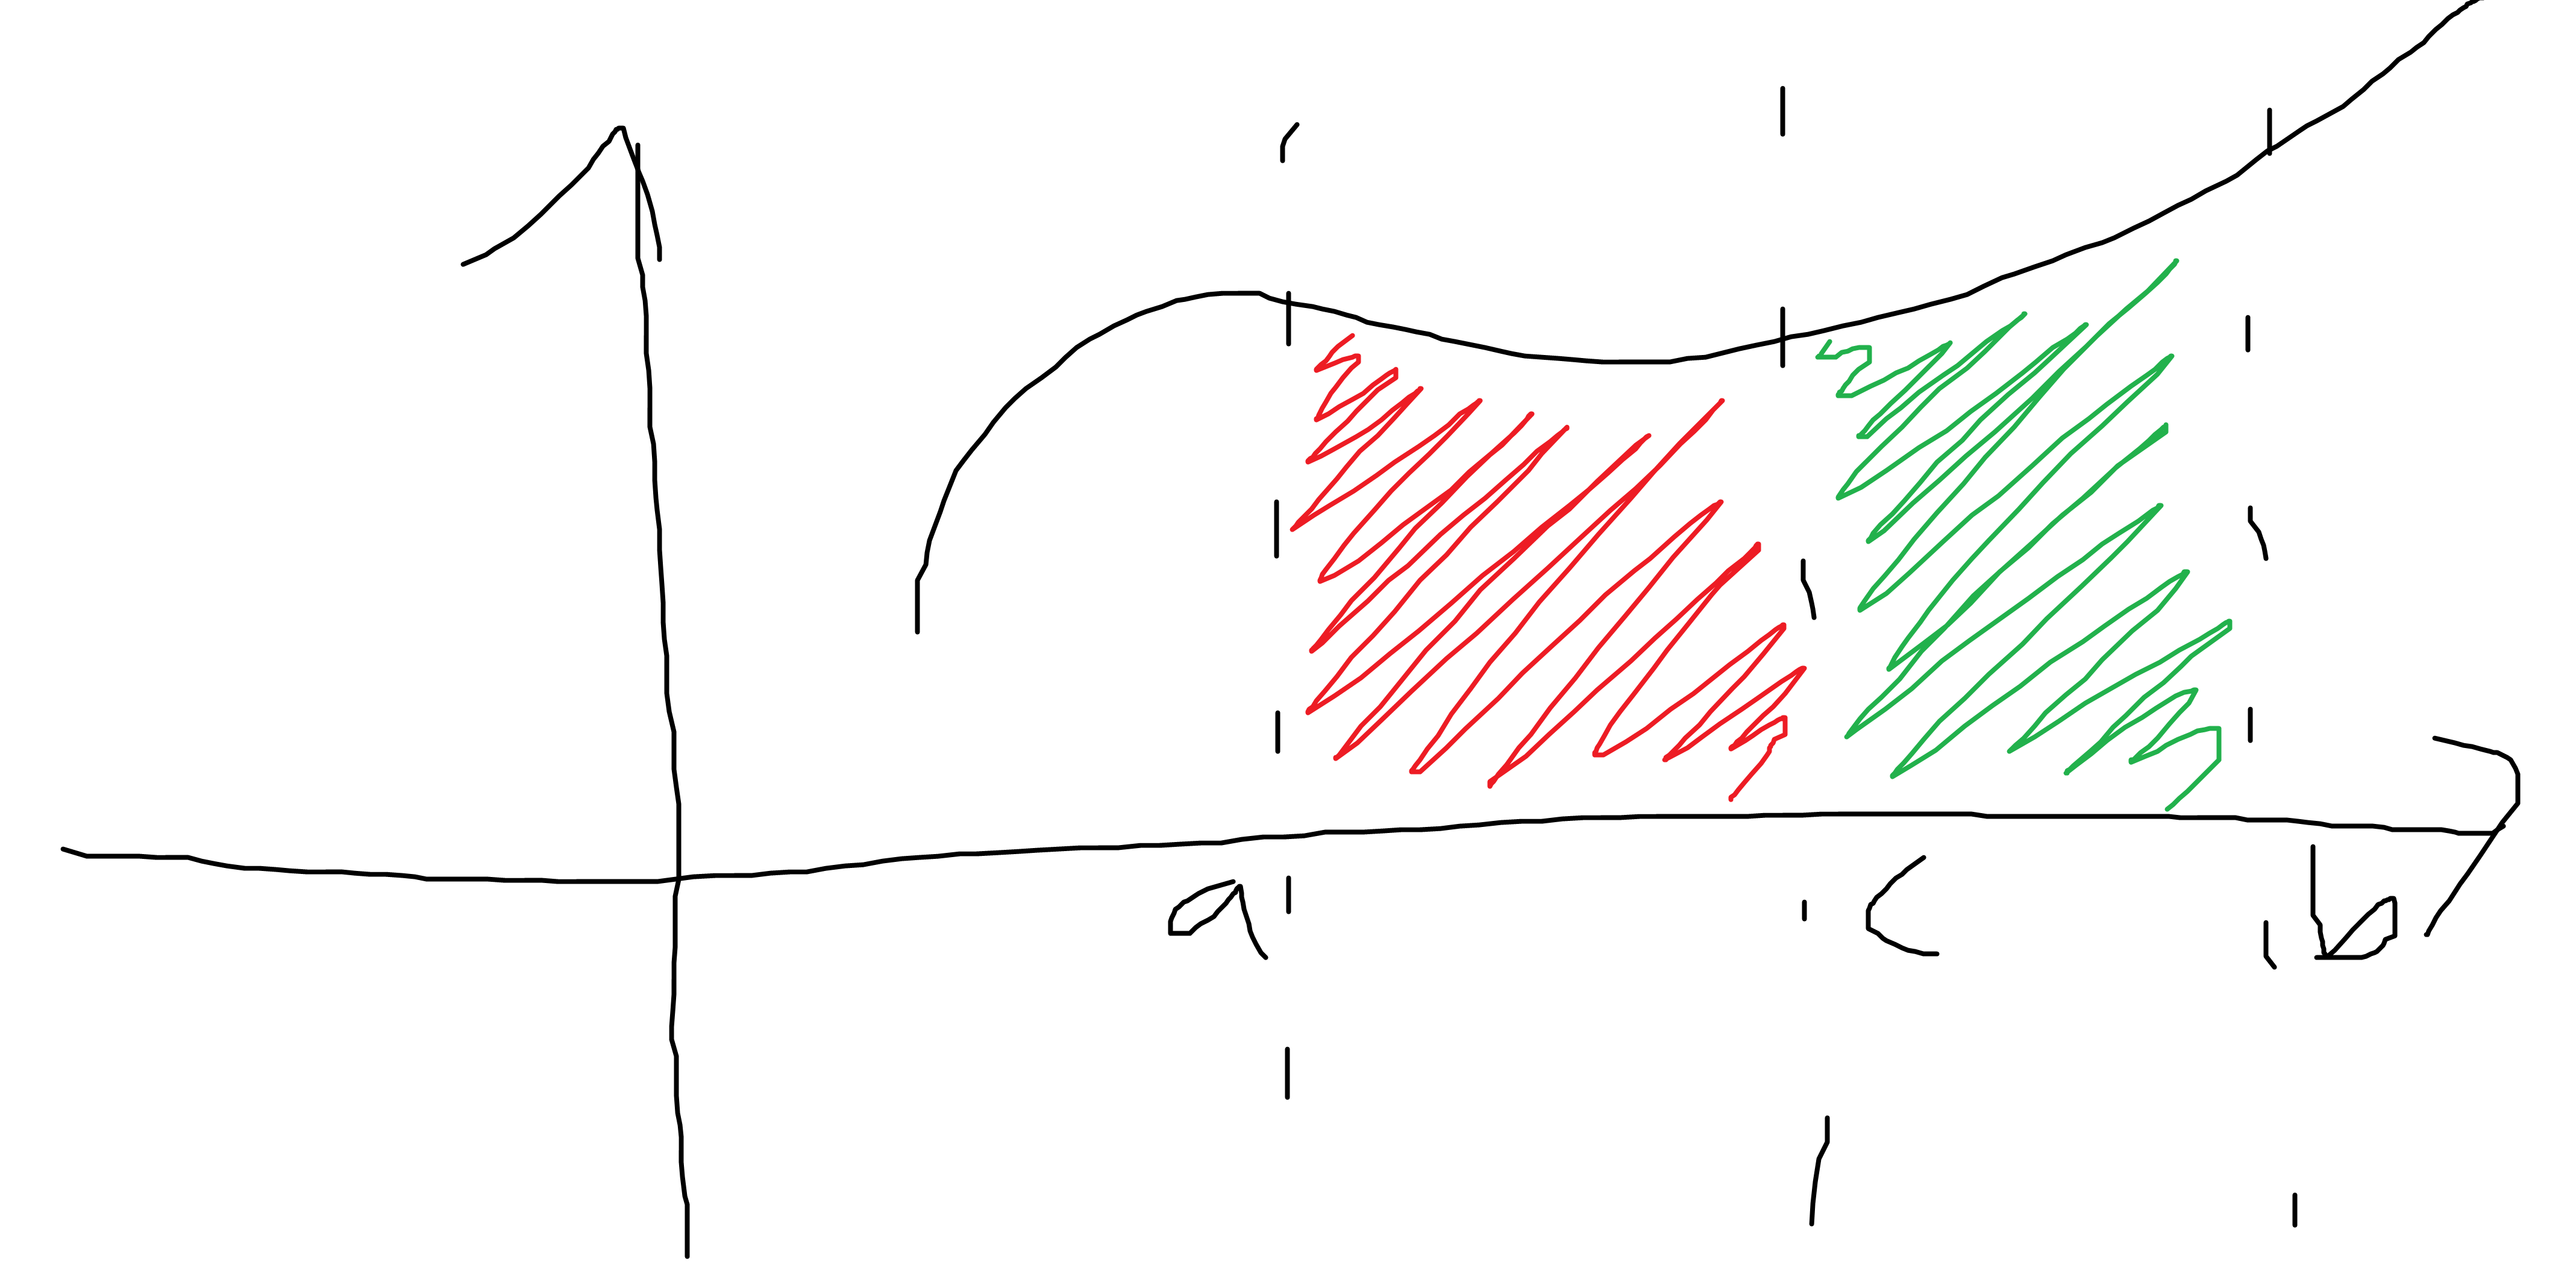
\includegraphics[height=3cm]{kepek/first.png}
		\caption{Paintben csináltam, dont hate. Zöld + piros = $\int_a^bf$}\label{}
	\end{figure}
	Eddig: $\int_a^bf:\quad a<b$
	\begin{definition}
		\[ \int_a^af:=0 \]
		Ha $a<b$ és $f\in R[a,b]$
		\[ \int_b^af:=-\int_a^bf \]
	\end{definition}
	\begin{theorem}
		Tegyük fel, hogy $f\in R[A,B],\quad a,b,c\in[A,B]$.
		\[ \int_a^bf=\int_a^cf+\int_c^bf \]
		\textit{bizonyítása meggondolandó.}
	\end{theorem}
	\subsection{Integrálható függvények osztálya}
	\begin{theorem}
		Ha $f\in k[a,b]$ monoton \quad $\Rightarrow\quad f\in R[a,b]$
		
		\textit{bizonyítás:} (oszcillációs összegekkel)
		
		Legyen $f$ (például) $\nearrow [a,b]$-n.
		\[ \tau:=\{ a=x_0<x_1<\ldots<x_n=b \}\in\mathcal{F}[a,b]\quad \text{tetszőleges} \]
		\[ \inf\{ f(x)\ | \ x_i\leq x\leq x_{i+1} \}=:m:=f(x_i) \]
		\[ \sup\{ f(x)\ | \ x_i\leq x\leq x_{i+1} \}=:M:=f(x_{i+1}) \]
		\[ \varOmega(f,\tau)=S(f,\tau)-s(f,\tau)=\sum_{i=0}^{n-1}M_i(x_{i+1}-x_i)\sum_{i=0}^{n-1}m_i(x_{i+1}-x_i)= \]
		\[ = \sum_{i=0}^{n-1}(M_i-m_i)(x_{i+1}-x_i)=\sum_{i=0}^{n-1}\overbrace{\left(f(x_{i+1})-f(x_i)\right)}^{\geq 0}\overbrace{(x_{i+1}-x_i)}^{\geq 0}\leq \max_{0\leq i\leq n-1}(x_{i+1}-x_i)\cdot\sum_{i=0}^{n-1}(f(x_{i+1})-f(x_i))\]
		\text{-- teleszkópikus!}
		\[ \Rightarrow\quad \varOmega(f,\tau)\leq ||\tau||\cdot (f(b)-f(a)) \]
		\[ \forall\varepsilon>0\quad \tau\in\mathcal{F}[a,b]:\quad ||\tau||\cdot\frac{\varepsilon}{f(b)-f(a)} \]
		\[ \Rightarrow\quad \varOmega(f,\tau)<\varepsilon\quad \Rightarrow\quad f\in R[a,b].\quad \blacksquare \]
	\end{theorem}
	\begin{theorem}
		Ha $f\in c[a,b]\quad \Rightarrow \quad f\in R[a,b]$, azaz:
		\[ C[a,b]\subset R[a,b] \]
		\textit{biz. nélkül. (ne gondoljuk meg!)}
	\end{theorem}
	\begin{theorem}
		Tegyük fel, hogy $f:[a,b]\to\R$ szakaszonként folytonos, azaz: 
		\[ \exists n\in\N,\quad \text{és}\quad \exists\tau=\{ a=x_0<...<x_n=b \}, \]
		\[ f\big|_{(x_i,x_{i+1})}\quad \text{folyt.}\quad (i=0,\ldots,n-1),\quad \text{és}\quad \exists\lim_{x_i\to0}f,\quad \lim_{x_{i+1}-0}f\quad \text{és végesek} \]
		Ekkor $f\in R[a,b]$, és
		\[ \int_a,b f= \sum_{i=0}^{n-1}\int_{x_i}^{x_{i+1}}f \]
	\end{theorem}
	
	\begin{figure}[H]
		\centering
		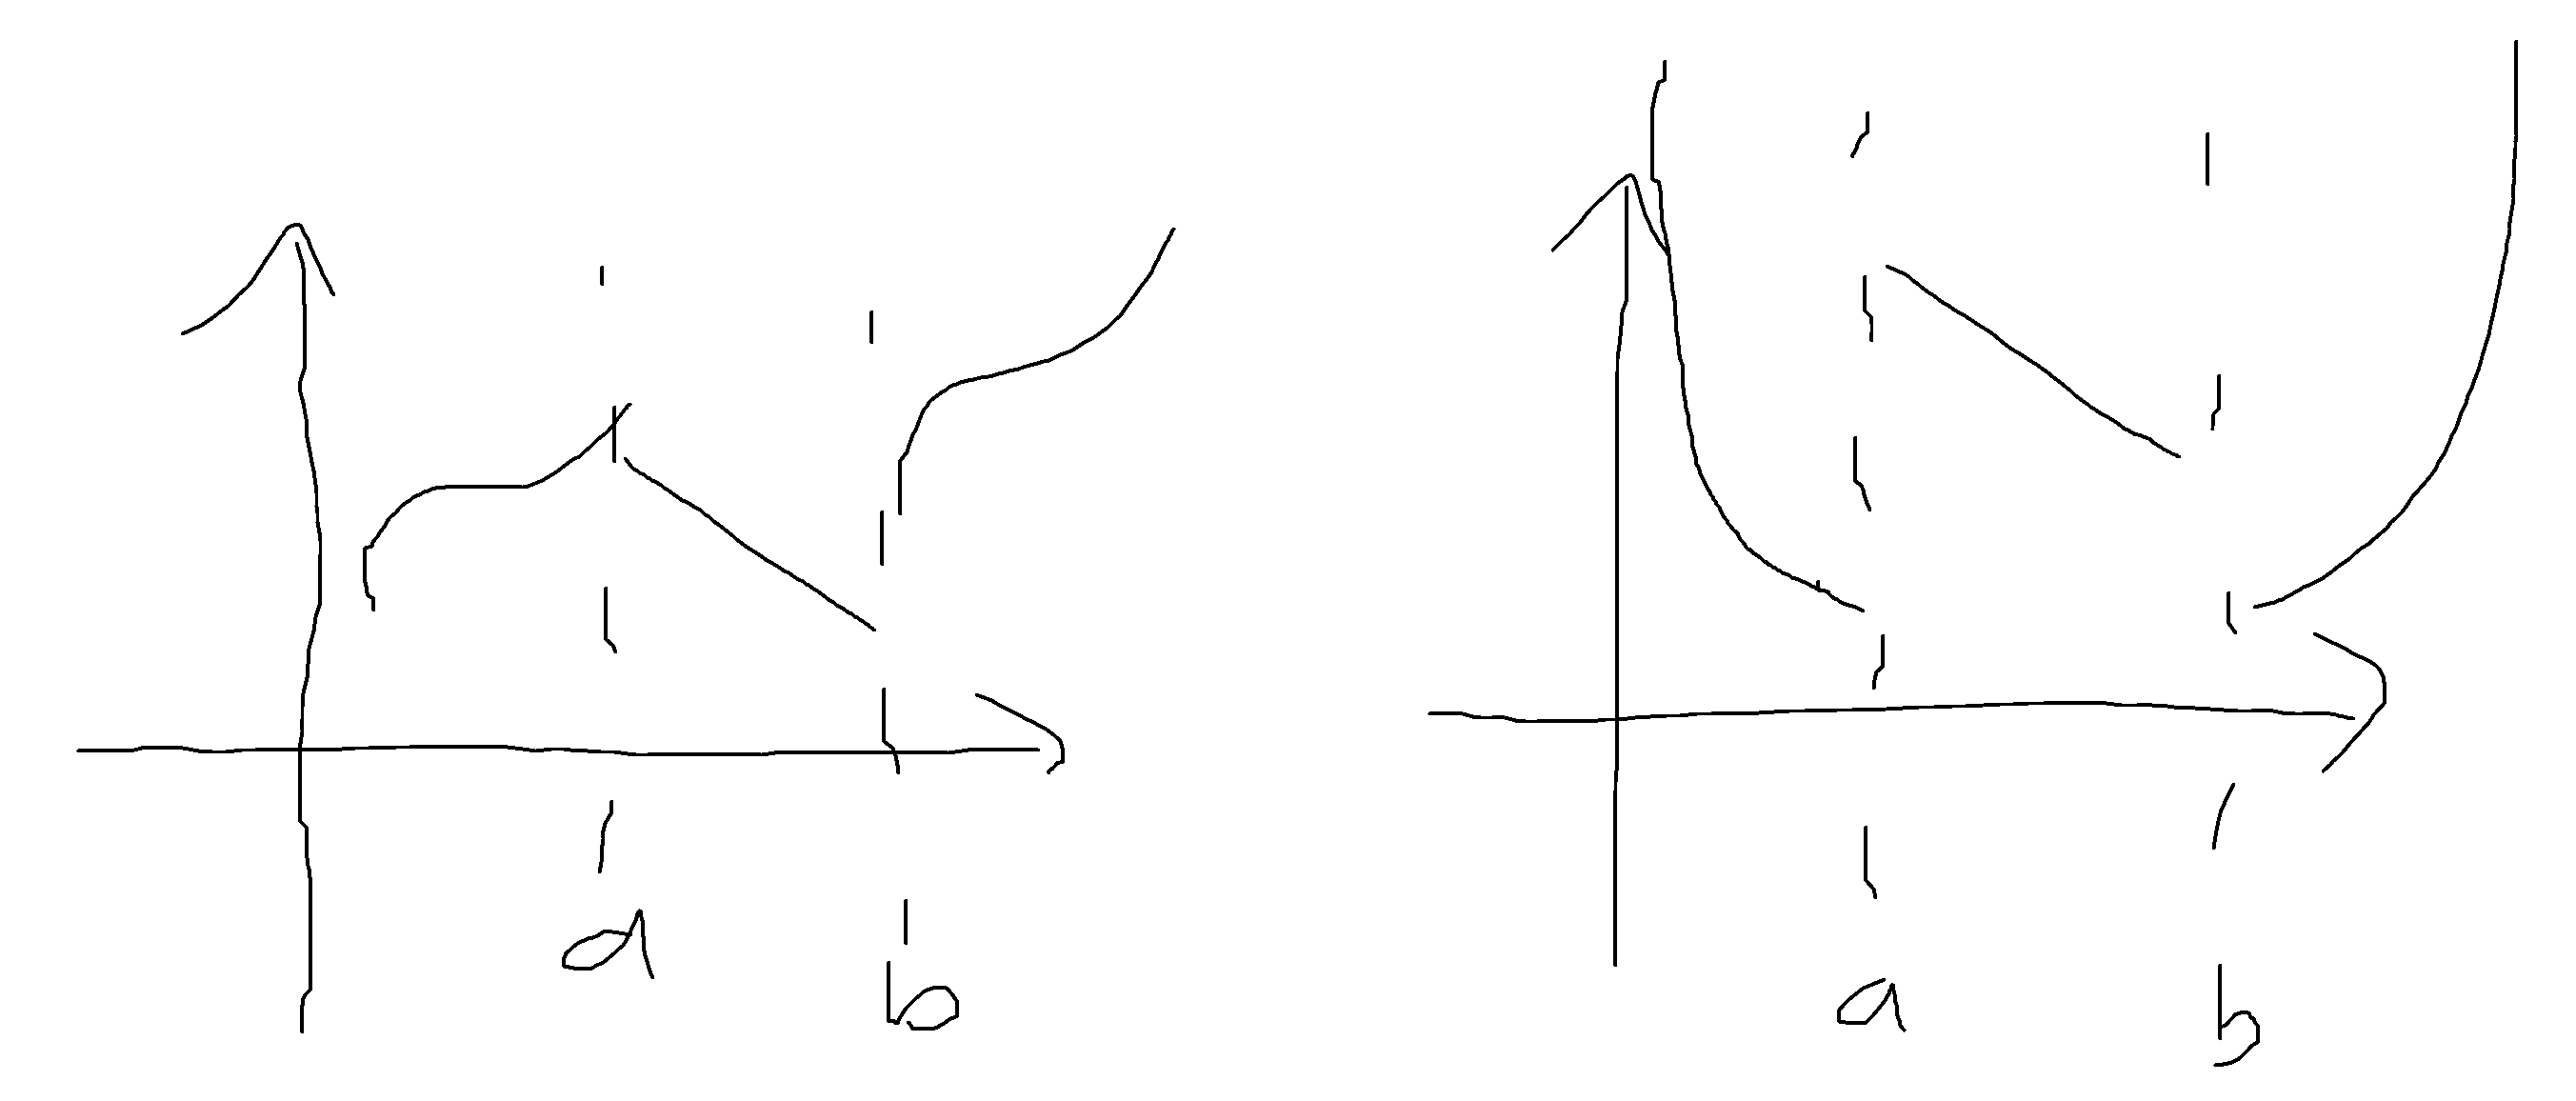
\includegraphics[height=3cm]{kepek/second.png}
		\caption{Szakaszos és nem szakaszos integrálhatóság (végtelen nem megengedett, ugye)}\label{}
	\end{figure}
	\subsection{Egyenlőtlenségek}
	\begin{theorem}
		\begin{enumerate}\
			
			\item Ha $f\in R[a,b]\quad \text{és}\quad f\geq0\quad \Rightarrow\quad \int_a^bf\geq0$
			\item Ha $f,g\in R[a,b]\quad \text{és}\quad f\geq g\quad \Rightarrow\quad \int_a^bf\leq\int_a^bg$
		\end{enumerate}
	\end{theorem}
	\begin{theorem}
		\[f\in R[a,b]\quad \Rightarrow\quad |f|\in R[a,b]\quad \text{és}\quad \left|\int_a^bf\right|\leq\int_a^b\left|f\right| \]
	\end{theorem}
	\begin{note}
		Visszafelé ez az állítás nem teljesül. Például:
		\[ f(x):=\begin{cases}
			1,\quad x\in\Q\\
			-1, x\in\Q^*
		\end{cases} \]
		$|f|\in R[0,1],\quad f\notin R[0,1].\quad \blacksquare$
	\end{note}
	\begin{theorem}
		(az integrál számítás első középértéktétele)
		
		Tegyük fel, hogy 
		\[ \left.\begin{gathered}
			f,g\in R[a,b]\\
			g\geq 0,\quad [a,b]\text{-n}\\
			\inf\mathcal{R}_f=:m,\quad \sup\mathcal{R}_f=:M\\
		\end{gathered}\right\}\quad \Rightarrow\quad m\int_a^bg\leq\int_a^bf\cdot g\leq M\int_a^bg.\]
		Ha még $f\in C[a,b]$ is teljesül,
		\[ \exists\xi[a,b]:\quad \int_a^bf\cdot g=f(\xi)\cdot\int_a^bg \]
	\end{theorem}
	\begin{theorem}
		(Cauchy - Bunyakovszkij)
		
		Tegyük fel, hogy $f,g\in R[a,b]$. Ekkor $f\cdot g\in R[a,b]$
		\[ \left|\int_a^bf\cdot g\right|\leq\sqrt{\int_a^b|f|^2}\cdot\sqrt{\int_a^b|g|^2} \]
		\textit{bizonyítás nélkül. (ezt se kell meggondolni!)}
	\end{theorem}
	\subsection{Az integrál kiszámítása}
	Eddig: Prím függvények nyílt intervallumon ért.
	\begin{definition}
		$a,b\in\R,\quad a<b.$ Az $F:[a,b]\to\R$ az $f:[a,b]\to\R$ egy primitív függvénye $[a,b]$-n, ha
		\[ F\quad \text{folytonos}\quad [a,b]\text{-n},\quad \text{és}\quad  F'(x)=f(x)\quad (\forall x\in(a,b)). \]
	\end{definition}
	\begin{theorem}
		(Newton-Leibniz)
		
		Tegyük fel, hogy
		\[ \left.\begin{gathered}
			f\in R[a,b]\\
			f\text{-nek van primitív függvénye}\quad [a,b]\text{-n}\\
		\end{gathered}\right\} \quad \Rightarrow\quad \int_a^bf=F(b)-F(a)=:[F(x)]_a^b  \]
		$F$ az $f$ egy primitív függvénye.
		\begin{note}
			Kapcsolat a differenciálszámítás és az integrálszámítás között.
		\end{note}
		\textit{Bizonyítás:} Legyen $\tau:=\{ a=x_0<x_1<\ldots<x_n=b \}\in\mathcal{F}[a,b]$ tetszőleges.
		\[ F(a)-F(b)=F(x_n)-F(x_0)\quad \overset{\text{TRÜKK}}{=}\quad (F(x_n)-F(x_{n-1}))+(F(x_{n-1})-F(x_{n-2}))+\ldots+(F(x_1)-F(x_0))=\]
		\[=\sum_{i=0}^{n-1}F(x_{i+1})-F(x_i)= \]
		Tegyünk gy apróbb megállapítást: $F$-re $[x_i,x_{i+1}]$-en a Lagrange k.é.t.: 
		\[ F(x_{i+1})-F(x_i)=F'(\xi_i)(x_{i+1}-x_i)\quad \overset{F'=f}{=}\quad f(\xi_i)(x_{i+1}-x_i) \]
		Folytatván a bizonyítást:
		\[ F(b)-F(a)=\sum_{i=0}^{n-1}f(\xi_i)(x_{i+1}-x_i) \]
		\[ \Downarrow \]
		\[ s(f,\tau)\leq F(b)-F(a)\leq S(f,\tau)\quad \inf\]
		$\forall \tau$-ra\quad $\Rightarrow\quad \sup$
		\[ I_*(f)\leq F(b)-F(a)\leq I^*(f) \]
		\[ f\in R[a,b]\quad \Rightarrow\quad I_*(f)=I^*(f)=\int_a^bf=\int_a^bf=F(b)-F(a).\quad \blacksquare \]
	\end{theorem}
	\begin{example}
		\[ f(x)=\sqrt{1-x^2}\quad |x|\leq 1 \]
		
		\begin{figure}[H]
			\centering
			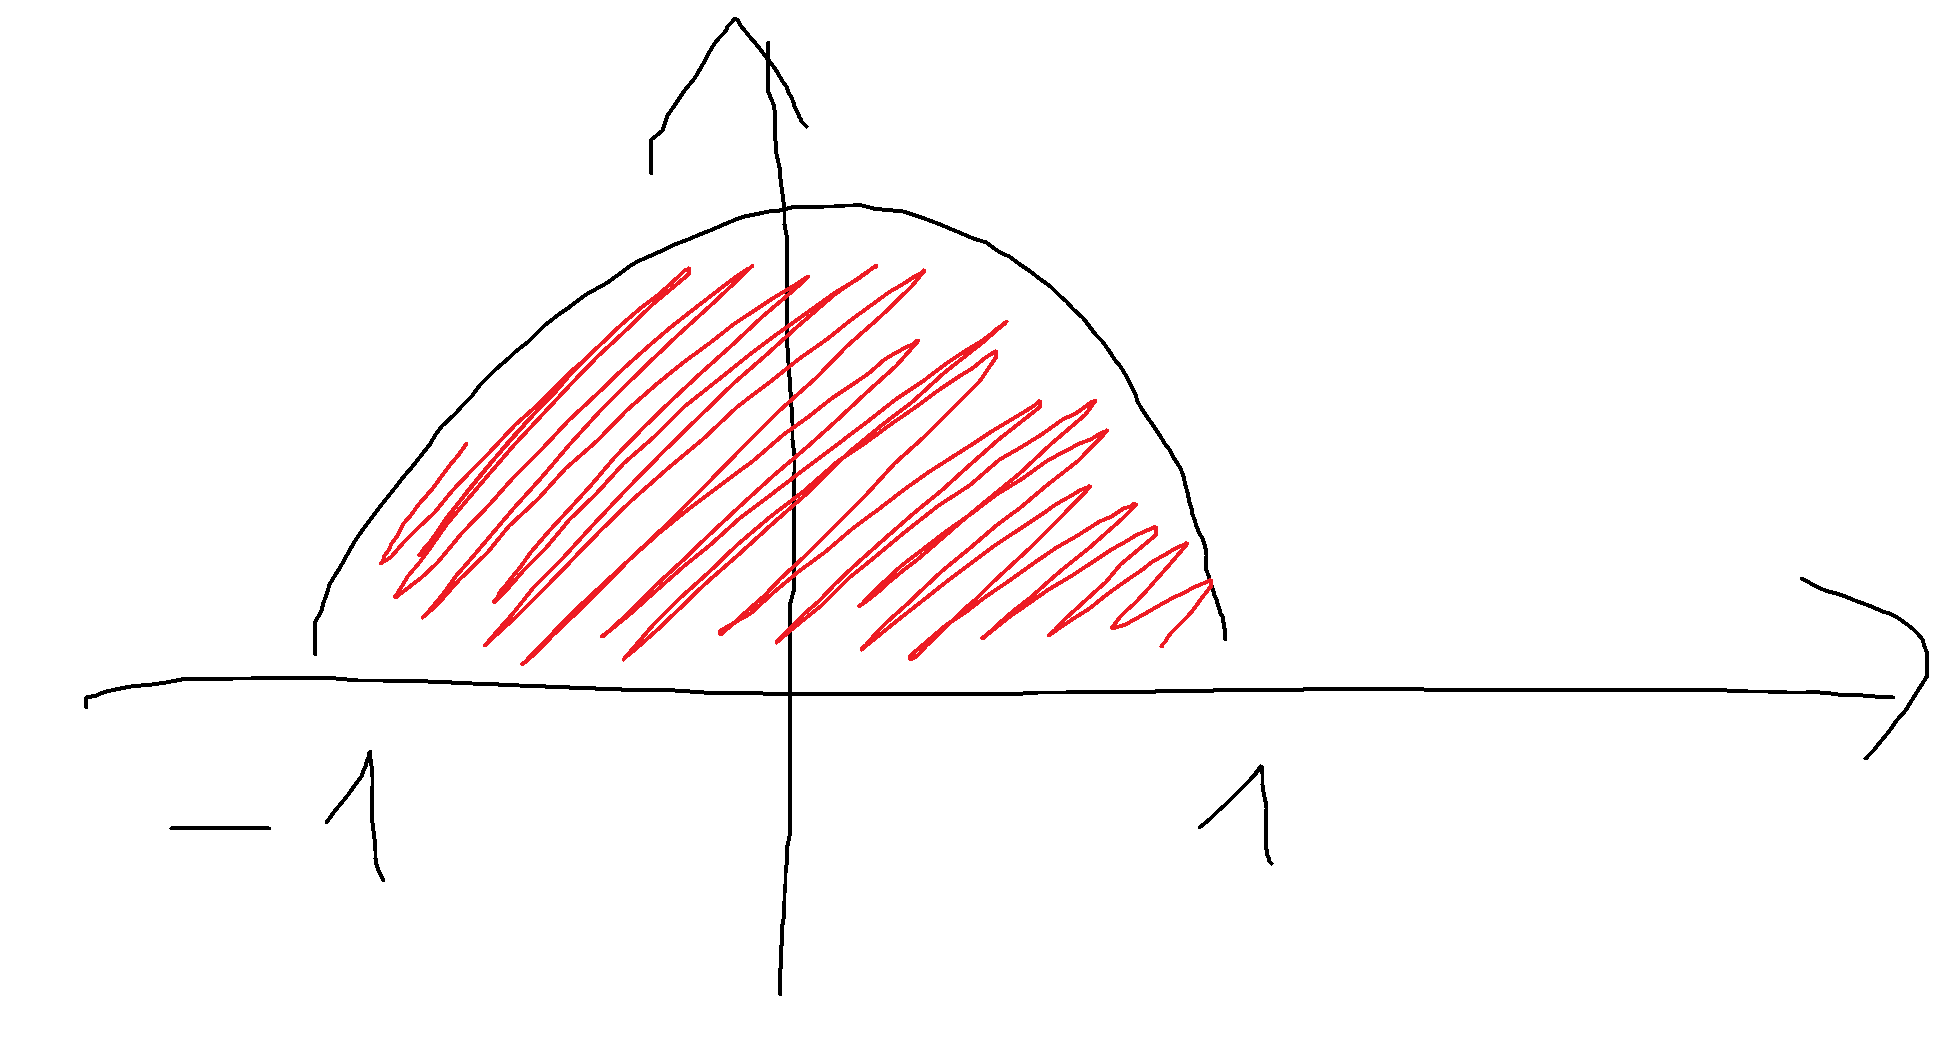
\includegraphics[height=3cm]{kepek/third.png}
			\caption{}\label{}
		\end{figure}
	\end{example}	
	A $\pi$ amit mi definiáltunk valóban ekvivalens, azzal, amit középsuliban tanultunk?
	\[ T=\int_{-1}^{1}\sqrt{1-x^2}\,dx=\left[\frac{\arc\sin x+x\sqrt{1-x^2}}{2}\right]_{-1}^1\quad \overset{\frac{\pi}{2}}{=}\quad \frac{\arc\sin1-\arc\sin(-1)}{2}=\frac{\pi}{2} \]
	Igen.
\end{document}
